%% This is file `DEMO-TUDaThesis.tex' version 3.28 (2022/11/15),
%% it is part of
%% TUDa-CI -- Corporate Design for TU Darmstadt
%% ----------------------------------------------------------------------------
%%
%%  Copyright (C) 2018--2022 by Marei Peischl <marei@peitex.de>
%%
%% ============================================================================
%% This work may be distributed and/or modified under the
%% conditions of the LaTeX Project Public License, either version 1.3c
%% of this license or (at your option) any later version.
%% The latest version of this license is in
%% http://www.latex-project.org/lppl.txt
%% and version 1.3c or later is part of all distributions of LaTeX
%% version 2008/05/04 or later.
%%
%% This work has the LPPL maintenance status `maintained'.
%%
%% The Current Maintainers of this work are
%%   Marei Peischl <tuda-ci@peitex.de>
%%   Markus Lazanowski <latex@ce.tu-darmstadt.de>
%%
%% The development respository can be found at
%% https://github.com/tudace/tuda_latex_templates
%% Please use the issue tracker for feedback!
%%
%% If you need a compiled version of this document, have a look at
%% http://mirror.ctan.org/macros/latex/contrib/tuda-ci/doc
%% or at the documentation directory of this package (if installed)
%% <path to your LaTeX distribution>/doc/latex/tuda-ci
%% ============================================================================
%%
% !TeX program = lualatex
%%

\documentclass[
	ngerman,
	ruledheaders=section,%Ebene bis zu der die Überschriften mit Linien abgetrennt werden, vgl. DEMO-TUDaPub
	class=report,% Basisdokumentenklasse. Wählt die Korrespondierende KOMA-Script Klasse
	thesis={type=report},% Dokumententyp Thesis, für Dissertationen siehe die Demo-Datei DEMO-TUDaPhd
	accentcolor=1c,% Auswahl der Akzentfarbe
	custommargins=false,% Ränder werden mithilfe von typearea automatisch berechnet
	marginpar=false,% Kopfzeile und Fußzeile erstrecken sich nicht über die Randnotizspalte
	BCOR=5mm,%Bindekorrektur, falls notwendig
	parskip=half-,%Absatzkennzeichnung durch Abstand vgl. KOMA-Script
	fontsize=11pt,%Basisschriftgröße laut Corporate Design ist mit 9pt häufig zu klein
%	logofile=example-image, %Falls die Logo Dateien nicht vorliegen
]{tudapub}


% Der folgende Block ist nur bei pdfTeX auf Versionen vor April 2018 notwendig
\usepackage{iftex}
\ifPDFTeX
	\usepackage[utf8]{inputenc}%kompatibilität mit TeX Versionen vor April 2018
\fi

%%%%%%%%%%%%%%%%%%%
%Sprachanpassung & Verbesserte Trennregeln
%%%%%%%%%%%%%%%%%%%
\usepackage[english, main=english]{babel}
\usepackage[autostyle]{csquotes}% Anführungszeichen vereinfacht

% Falls mit pdflatex kompiliert wird, wird microtype automatisch geladen, in diesem Fall muss diese Zeile entfernt werden, und falls weiter Optionen hinzugefügt werden sollen, muss dies über
% \PassOptionsToPackage{Optionen}{microtype}
% vor \documentclass hinzugefügt werden.
\usepackage{microtype}

%%%%%%%%%%%%%%%%%%%
%Literaturverzeichnis
%%%%%%%%%%%%%%%%%%%
\usepackage[backend=biber,style=ieee,sorting=none]{biblatex}   % Literaturverzeichnis
\addbibresource{references.bib}


%%%%%%%%%%%%%%%%%%%
%Paketvorschläge Tabellen
%%%%%%%%%%%%%%%%%%%
%\usepackage{array}     % Basispaket für Tabellenkonfiguration, wird von den folgenden automatisch geladen
\usepackage{tabularx}   % Tabellen, die sich automatisch der Breite anpassen
%\usepackage{longtable} % Mehrseitige Tabellen
%\usepackage{xltabular} % Mehrseitige Tabellen mit anpassbarer Breite
\usepackage{booktabs}   % Verbesserte Möglichkeiten für Tabellenlayout über horizontale Linien

%%%%%%%%%%%%%%%%%%%
%Paketvorschläge Mathematik
%%%%%%%%%%%%%%%%%%%
%\usepackage{mathtools} % erweiterte Fassung von amsmath
%\usepackage{amssymb}   % erweiterter Zeichensatz
\usepackage{siunitx}   % Einheiten
\usepackage{subcaption}

% Paketvorschläge Grafiken
\usepackage{amsmath}
\usepackage{graphicx}
\usepackage{float}
\usepackage{tabularx}
\usepackage{booktabs}

%Formatierungen für Beispiele in diesem Dokument. Im Allgemeinen nicht notwendig!
\let\file\texttt
\let\code\texttt
\let\tbs\textbackslash
\let\pck\textsf
\let\cls\textsf

\usepackage{pifont}% Zapf-Dingbats Symbole
\newcommand*{\FeatureTrue}{\ding{52}}
\newcommand*{\FeatureFalse}{\ding{56}}

\begin{document}

\Metadata{
	title=Exploration of Acoustic Body
Signals and Their Detectability
Using 3D-Printed Ferroelectret
Sensors,
	author=Niels Haßler,
}

\title{Exploration of Acoustic Body
Signals and Their Detectability
Using 3D-Printed Ferroelectret
Sensors
}
\subtitle{A Study on Signal Origins, Frequency Ranges, and Comparison with Existing Measurement
Approaches}
\author[N. Haßler]{Niels Haßler}%optionales Argument ist die Signatur,
\birthplace{Geburtsort}%Geburtsort, bei Dissertationen zwingend notwendig
\reviewer{Stephan Schaumann \and Julian Seiler }%Gutachter

%Diese Felder werden untereinander auf der Titelseite platziert.
%\department ist eine notwendige Angabe, siehe auch dem Abschnitt `Abweichung von den Vorgaben für die Titelseite'
\department{etit} % Das Kürzel wird automatisch ersetzt und als Studienfach gewählt, siehe Liste der Kürzel im Dokument.
\group{Measurement and Sensor Technology Group}

\submissiondate{\today}
\examdate{\today}

% Hinweis zur Lizenz:
% TUDa-CI verwendet momentan die Lizenz CC BY-NC-ND 2.0 DE als Voreinstellung.
% Die TU Darmstadt hat jedoch die Empfehlung von dieser auf die liberalere
% CC BY 4.0 geändert. Diese erlaubt eine Verwendung bearbeiteter Versionen und
% die kommerzielle Nutzung.
% TUDa-CI wird im nächsten größeren Release ebenfalls diese Anpassung vornehmen.
% Aus diesem Grund wird empfohlen die Lizenz manuell auszuwählen.
%\tuprints{urn=XXXXX,printid=XXXX,year=2022,license=cc-by-4.0}
% To see further information on the license option in English, remove the license= key and pay attention to the warning & help message.

% \dedication{Für alle, die \TeX{} nutzen.}

\maketitle

\tableofcontents

\chapter{Introduction}
The human body emits acoustic signals that can provide valuable insights into a vast array of physiological
and pathological processes. Ranging from the rhytmic beating of the heart to subtle sounds produced
by the respiratory system and gastrointestinal tract or high frequency hits in joints, these signals offer a
non-invasive window into the body’s inner workings. Auscultation as one of the oldest diagnostic techniques,
has been used since the days of Hippocrates (c.460 - c.370 BC) to assess the health of patients by listening
to their internal sounds \cite{montinari_first_2019}. With the advent of modern sensor technology and advanced signal processing
techniques the analysis of acoustic body signals has exceeded far beyond the capabilities of the traditional
stethoscope and limited human hearing.
This work explores the origins of various acoustic body signals and their respective spectrums. Providing
excerpts of the physiological processes that generate these sounds and how they can be used for diagnostic
analysis.
In the second part of this work, an overview of in use and emerging sensor technologies for acoustic
emissions is given, focusing on their working principles and frequency ranges. Lastly, the detectability of
acoustically emitted signals using 3D-printed ferroelectret sensors is discussed and compared to existing
measurement approaches.
\chapter{Origins of Acoustic Body Signals}
In this chapter the origins of acoustic body signals are explored. A focus on cardiac and vascular sounds is given first. 
Next gastrointestinal and respariratory sounds are discussed. Finally, acoustic emissions from joints, tendons and muscles are covered.
For all signal types, the physiological processes that generate theses sounds are described and characterised by their frequency content. 
If research exists on diagnostic capabalities or pathophysiological alterations of these signals it is covered in the respective sections. 

\section{Cardiac and Vascular Sounds}
In a regular cardiac cycle the human heart emits sounds during two dominant events named the First Heart
Sound (S1) and Second Heart Sound (S2) \cite{debbal_computerized_2008}. S1 is generated by the closure
of the mitral and triscupid valves at the onset of systole, while S2 stems from the halting of the aortic
and pulmonary valves forcing a sudden deceleration of blood flow in the aorta and pulmonary artery, at the end of systole \cite{li_review_2020,debbal_computerized_2008}. 
Both actions form vibrations on the entire cardiac structure and surrounding tissues, which can then be detected as acoustic signals on the chest wall. 
Clinical practice has revealed a total of 5 positions on the chest wall where sounds can be best auscultated. 
\\

\begin{figure}[H]
\centering
\begin{subfigure}[t]{0.4\textwidth}
\centering
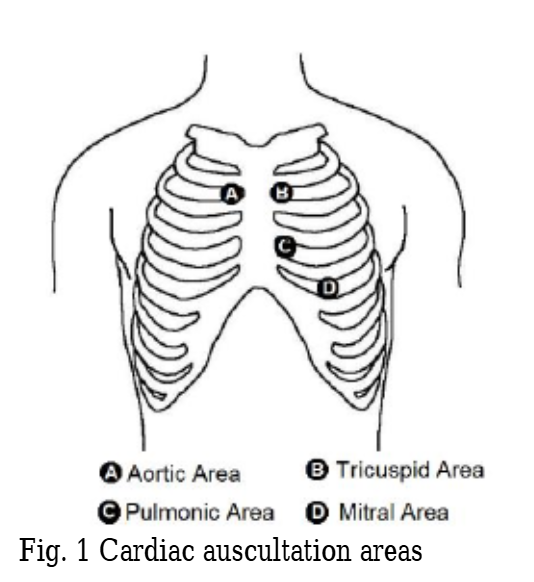
\includegraphics[width=\linewidth]{images/image.png}
\caption{}
\label{fig:left}
\end{subfigure}
\hfill
\begin{subfigure}[t]{0.4\textwidth}
\centering
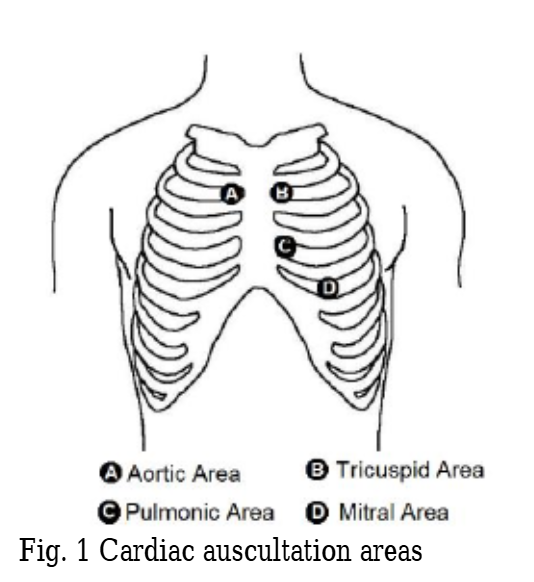
\includegraphics[width=\linewidth]{images/image.png}
\caption{ 1: Aortic valve, 2: Pulmonary valve, 3: Tricuspid valve, 4: Mitral valve, 5: Erb's point}
\label{fig:right}
\end{subfigure}
\label{fig:double}
\caption{(a) Valves of the human heart  and (b) Cardiac auscultation points on the chest wall}
\end{figure}

Using Phonocardiography (PCG) the acoustic signals of the heart can be recorded and analyzed for diagnostic purposes. In the time-domain, S1 correspond to the QRS complex of the electrocardiogram (ECG) and S2 to the T-wave. 
A normal PCG signal has a frequency content in the range of \SIrange{40}{200}{\hertz} \ \cite{li_review_2020}. S1 typically lasts around \SIrange{50}{100}{m\second} with a power spectrum in the range of \SIrange{50}{150}{\hertz}. 
S2 is shorter, lasting around \SIrange{25}{50}{m\second} and has a higher frequency content in the range of \SIrange{50}{200}{\hertz}, which is expected as less blood is present in the cardiac chambers. 

\begin{figure}[H]
\centering
\begin{subfigure}[t]{0.4\textwidth}
\centering
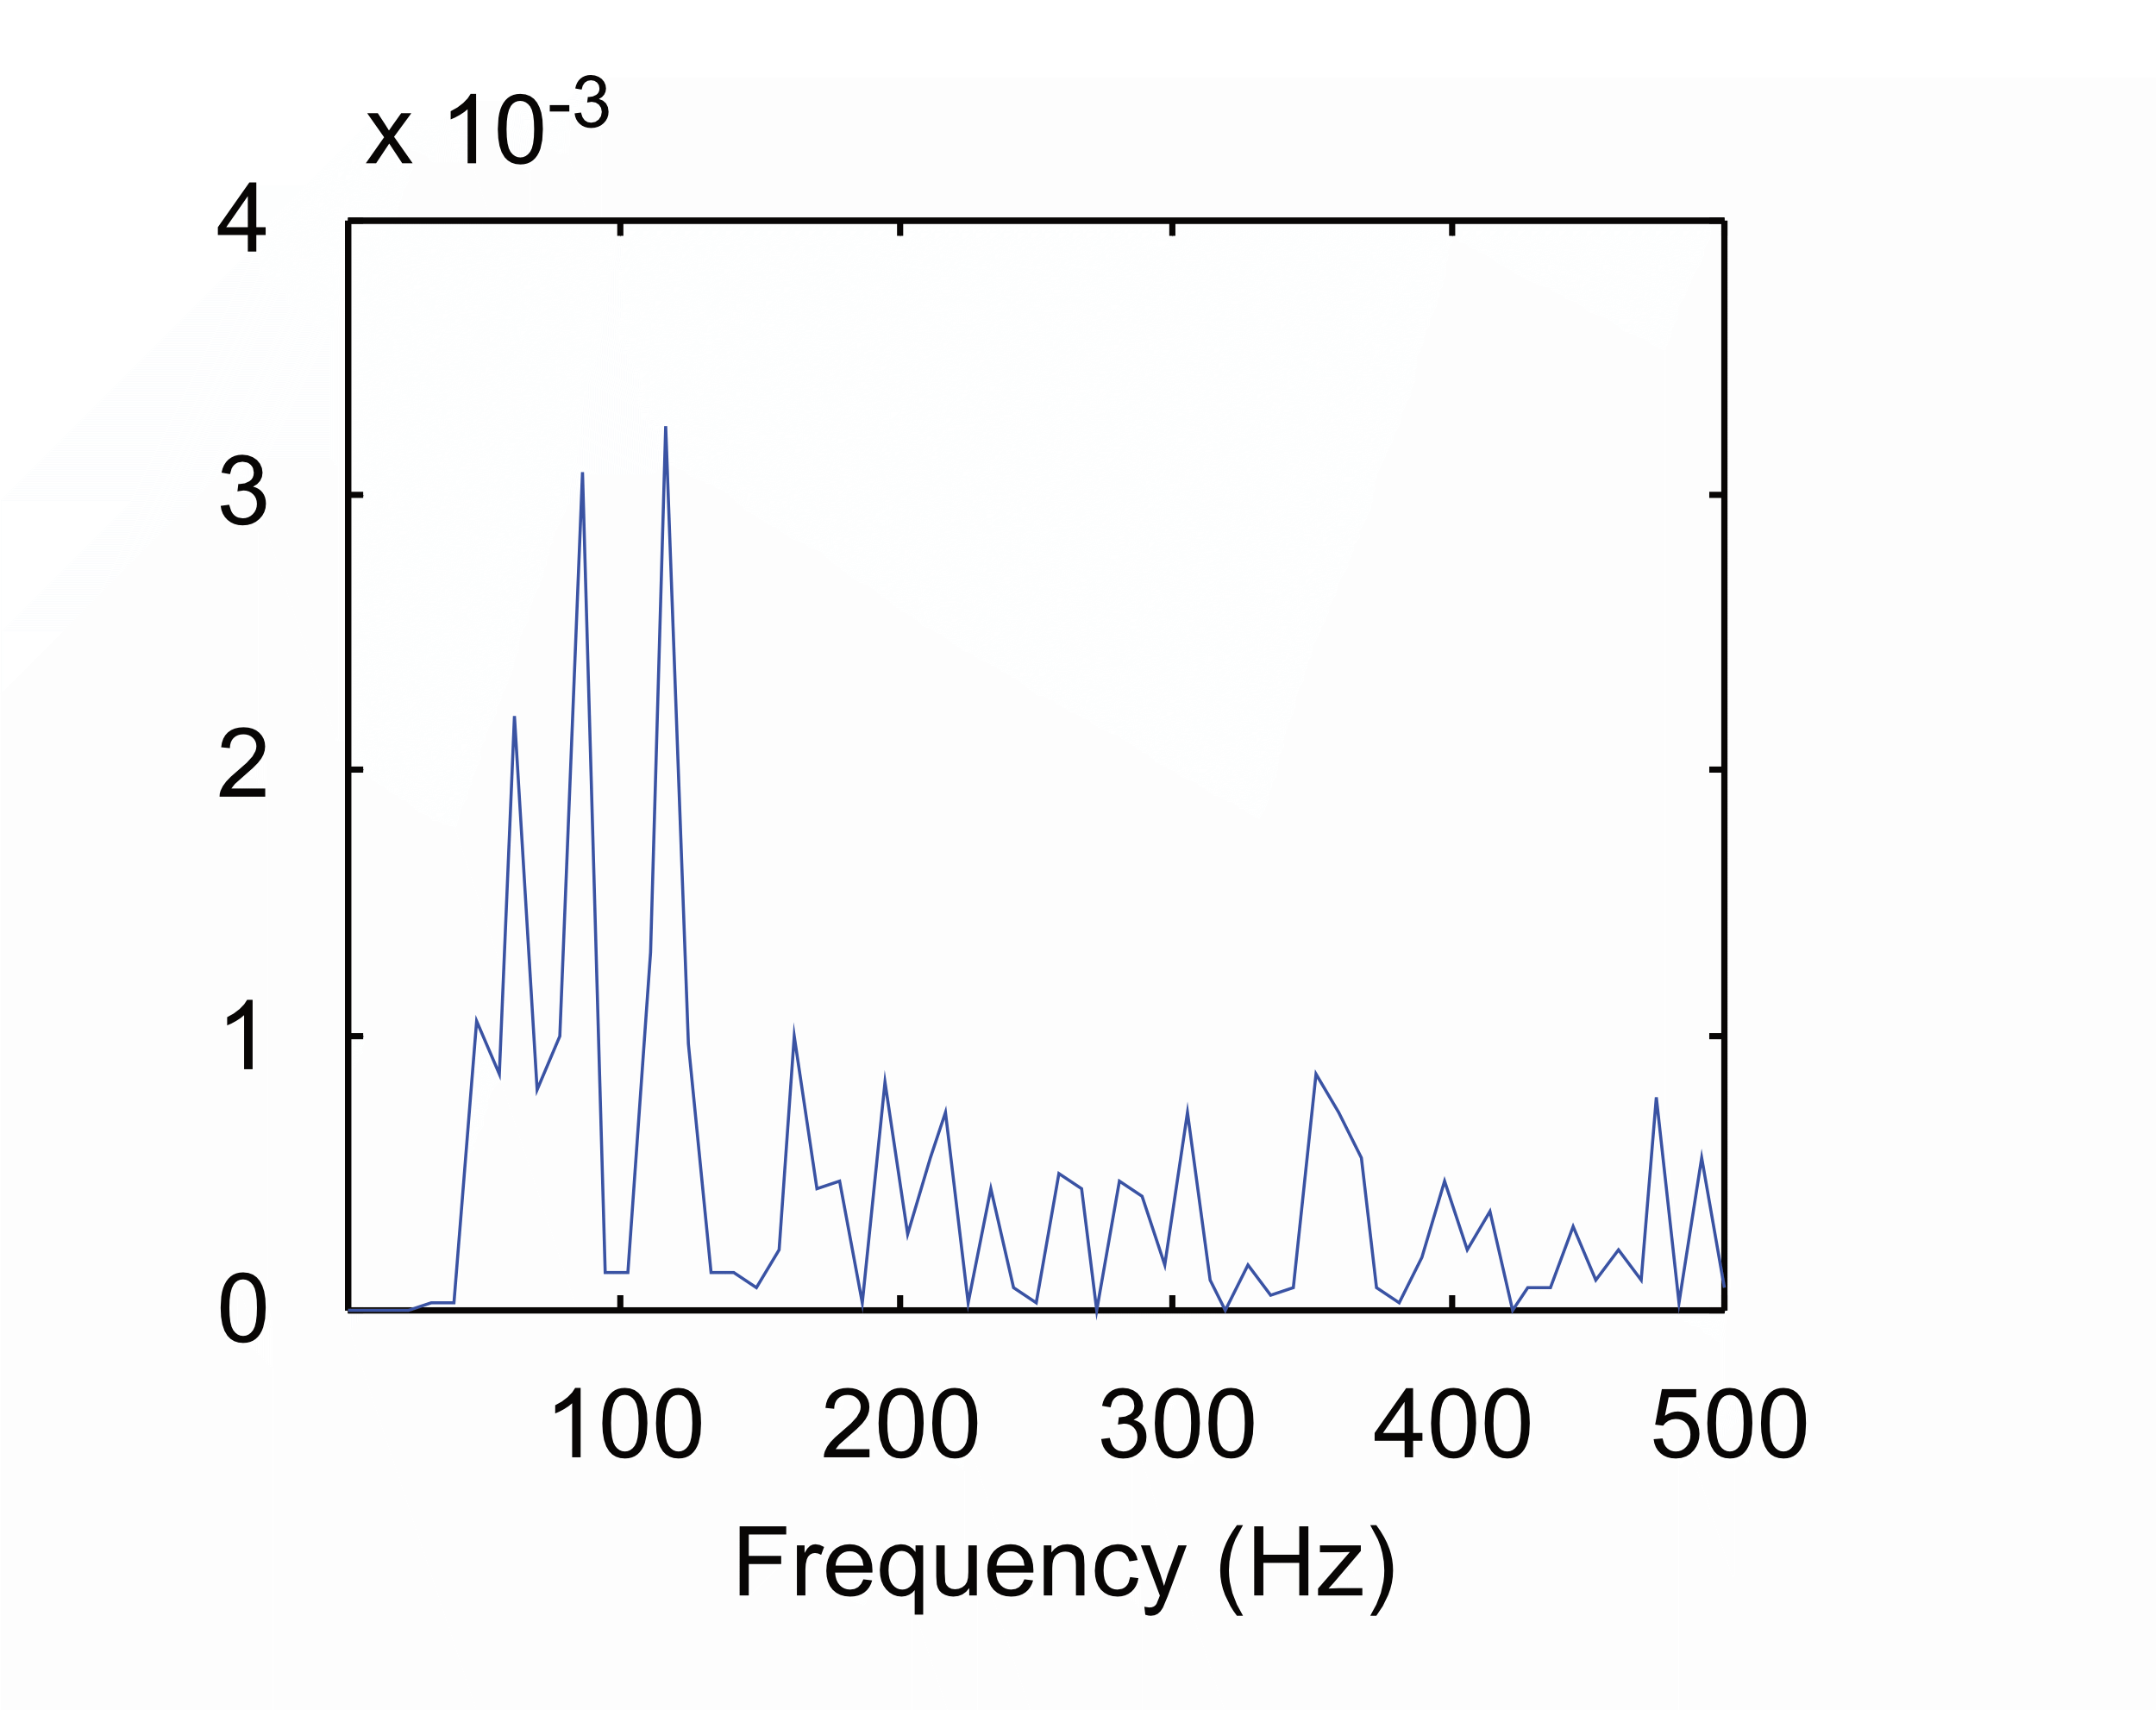
\includegraphics[width=\linewidth]{images/S1-Spectrum.png}
\caption{Frequency spectrum for the sound S1}
\label{fig:left}
\end{subfigure}
\hfill
\begin{subfigure}[t]{0.4\textwidth}
\centering
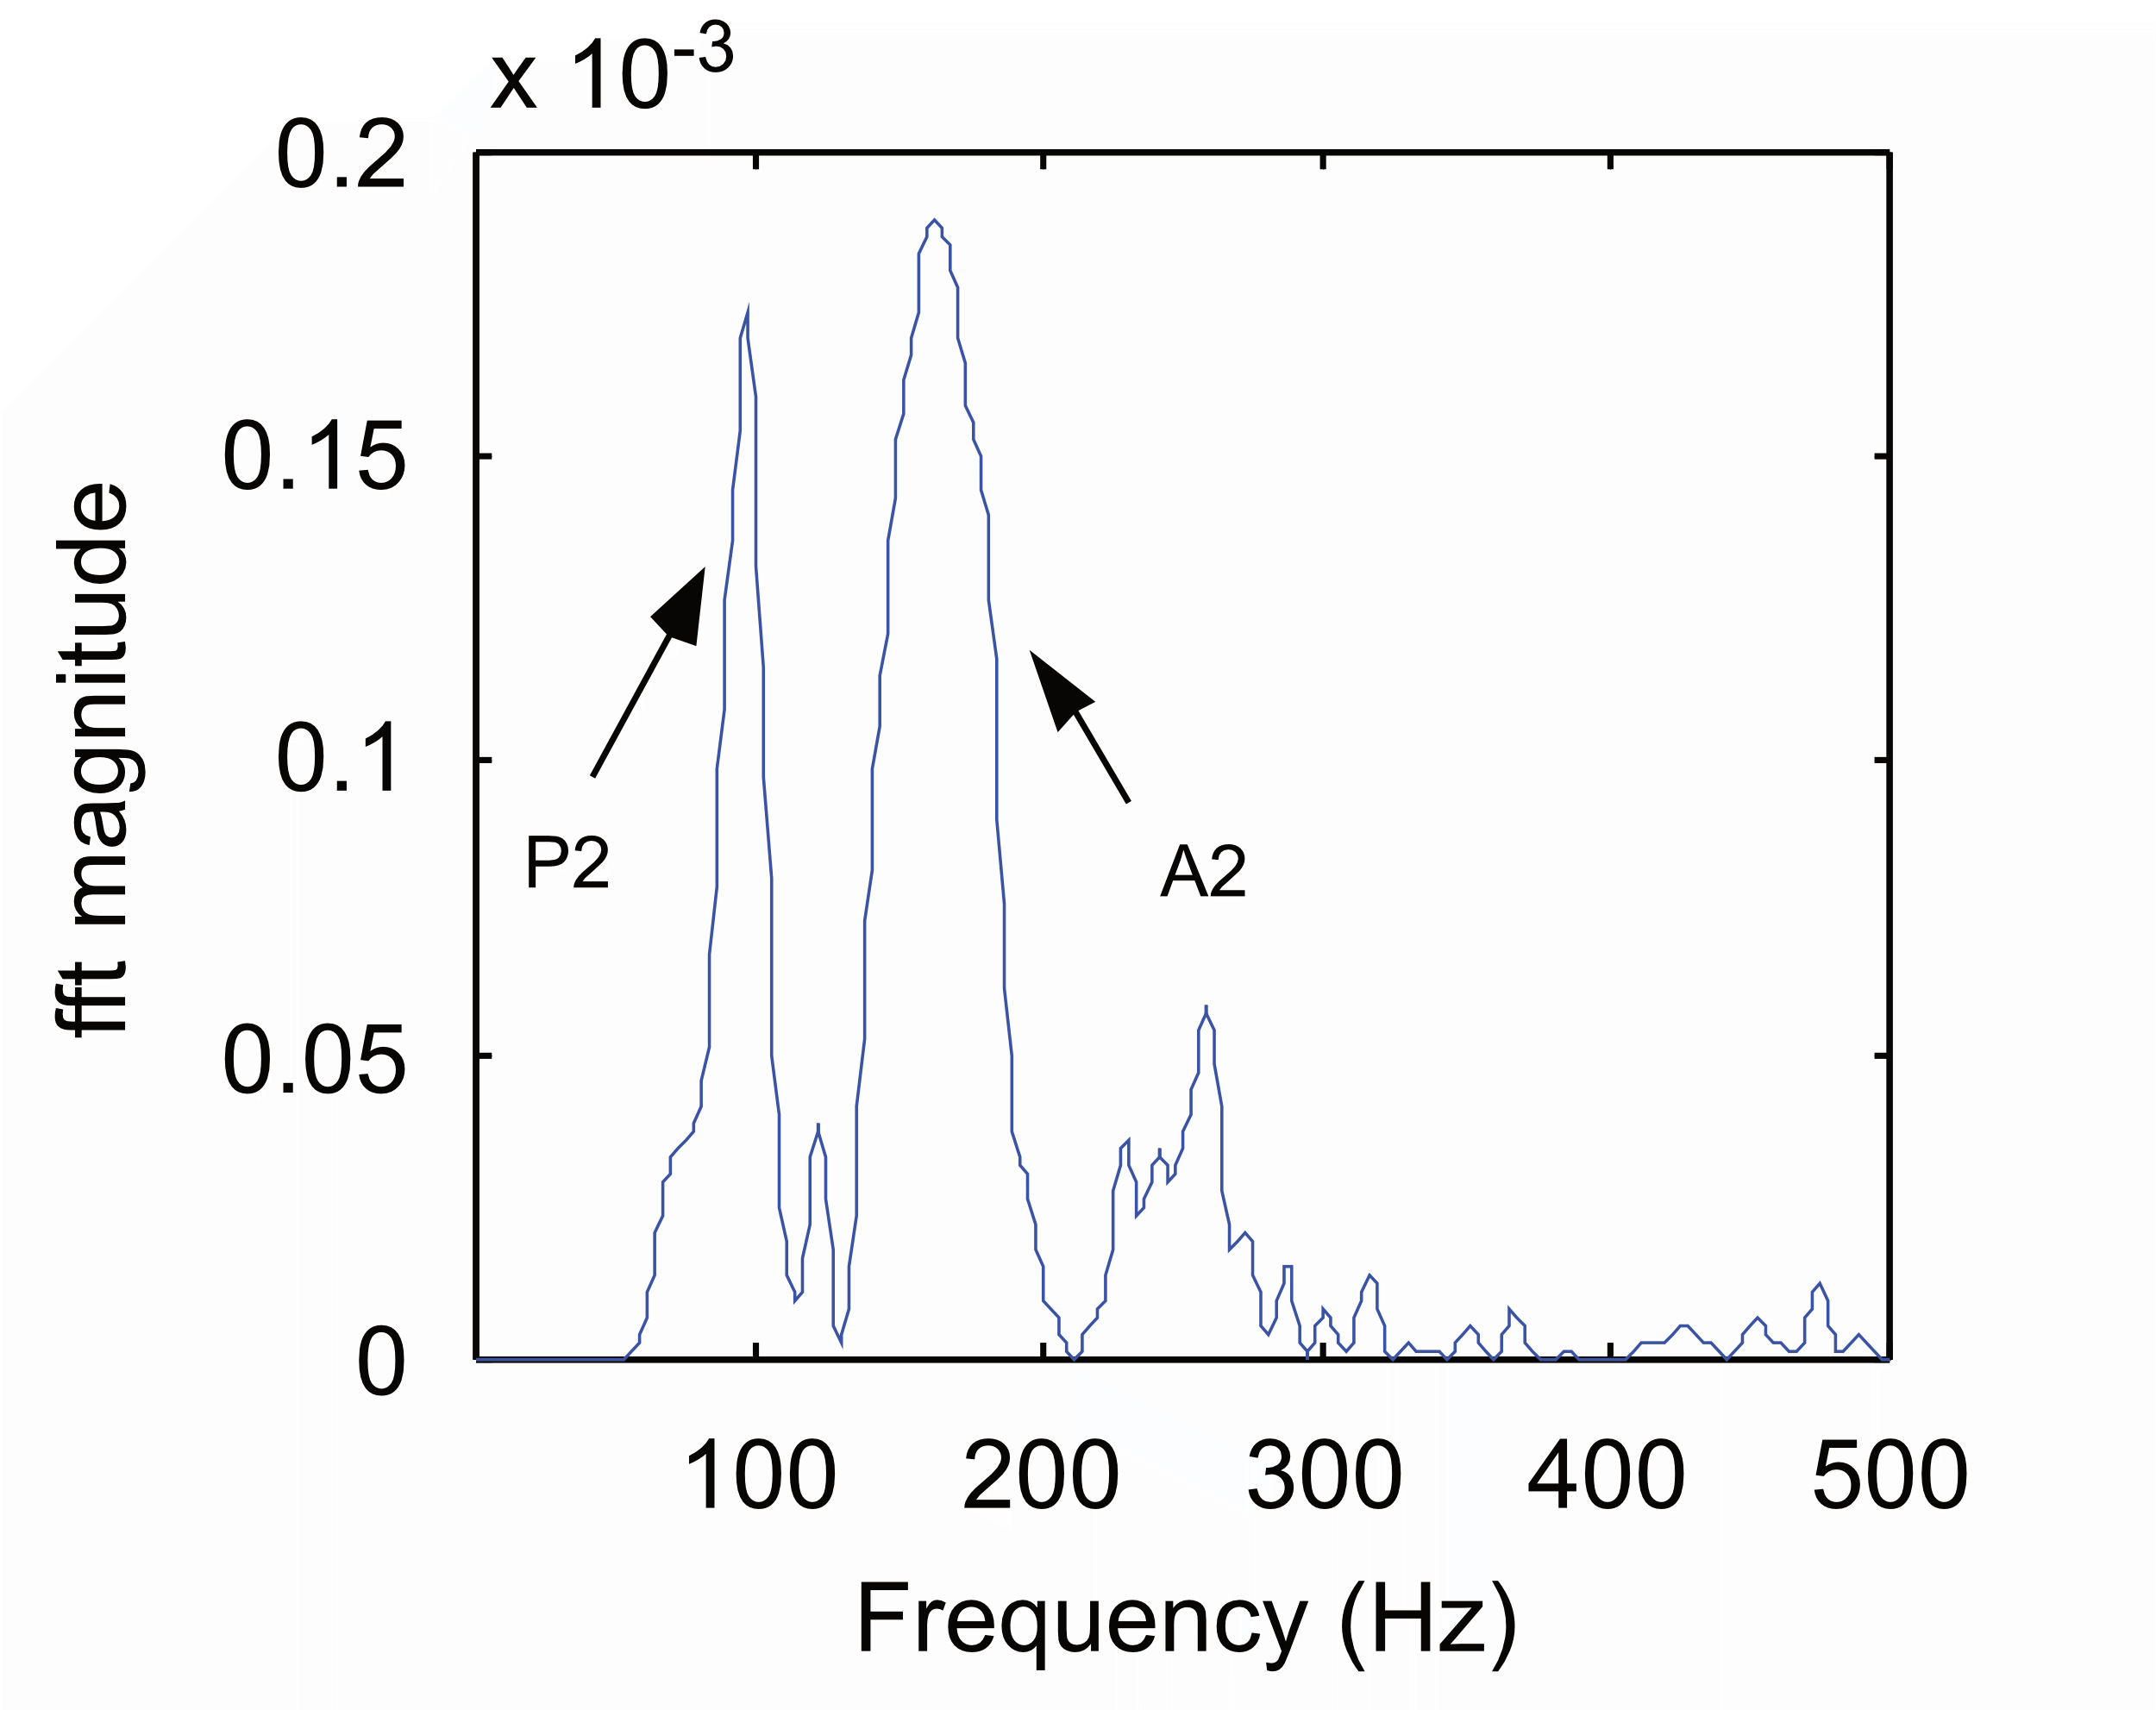
\includegraphics[width=\linewidth]{images/S2-Spectrum.png}
\caption{Frequency spectrum for the sound S2 }
\label{fig:right}
\end{subfigure}
\label{fig:double}
\caption{Graphs from S.M.Debbal et al. \cite{debbal_computerized_2008} , (b) shows the spectral decomposition of the sound S2, where the first peak corresponds to the aortic valve and the second to the pulmonary valve.}

\end{figure}

The spectral shape of S1 and S2 are influenced by body surface area, sex and blood pressure, ventricular mass and thus may change due to disease \cite{li_review_2020,chan_haemodynamic_2013}.
Furthermore in pathologocial conditions additional heart sounds may be observed, such as the Third and Fourth Heart Sound (S3 and S4) or high frequency murmurs ranging from \SIrange{600}{1000}{\hertz} \cite{ren_novel_2018}.
\\\\
Diseases in the vascular system can too produce acoustic signals. 
Turbulent blood flow in arteries caused by stenosis, aneurysms or arteriovenous malformations cause high pressure fluctuations in the post-stenotic region. 
Through the interaction of the vessel wall with the fluctuating blood flow, vibrations are generated and transmitted to the body surface \cite{kirkeeide_wall_1977}.
The frequency content of these sounds is typically in the range of \SIrange{100}{300}{\hertz}, more severe stenosis (>70\%) can produce sounds up to \SI{1000}{\hertz} \cite{khalili_spectral_2021}.

\section{Gastrointestinal Sounds}
Phonoenterography (PEN) is the recording and analyis of acoustic signals produced by the gastrointestinal (GI) tract. 
Healthy PEN signals consist of a continous isolated and short events in a frequency range of up to \SI{1500}{\hertz}  with the majority of energy located between \SIrange{50}{2500}{\hertz} \cite{ranta_digestive_2010-2}.
\\Two approaches exist for interpreting PEN signals. The first is based on the analysis of the indivual sounds and their categorisation \cite{dimoulas_bowel-sound_2008}.
The second approach is based on the analysis of the overall acoustic activity, like mean sound duration, silence between
sounds duration, signal energy etc. The weighted combination of these features form the Acoustic Activity Index (AAI) \cite{ranta_digestive_2010-2}.
Using the AII, the digestive activity of the GI tract can be assessed and thus used for diagnostic purposes and long term monitoring.

\section{Respiratory Sounds}
The respiratory cycle consist of two main phases - inspiration and expiration. Normal adults breathe 16-20 Times per minute. 
A healthy lung produces sounds during both phases. In inspiration sound is generated through turbulent flow in the lobar and segemental airways, in expiration sound arises from more central airways. 
Frequency ranges from \SIrange{50}{2500}{\hertz} \cite{andres_respiratory_2018}, with the majority of energy in the range of \SIrange{50}{2500}{\hertz}\cite{pasterkamp_respiratory_1997}.

When deciding on sensor position for the detection of respiratory sounds, it is important to consider that the primary pathway for transmitted sound changes with frequency \cite{pasterkamp_respiratory_1997}.
Lung parenchyma and tissue act as a low-pass filter and direct coupling to the chest wall is dominant. Thus transmission below 300Hz provides information mostly on lung parenchyma or thoracic cavity. 
Higher frequencies take the airway lumen route \cite{mahagnah_gas_1995} and are thus best detected at the trachea or neck.
\begin{figure}[H]
\centering
\begin{subfigure}[t]{0.4\textwidth}
\centering
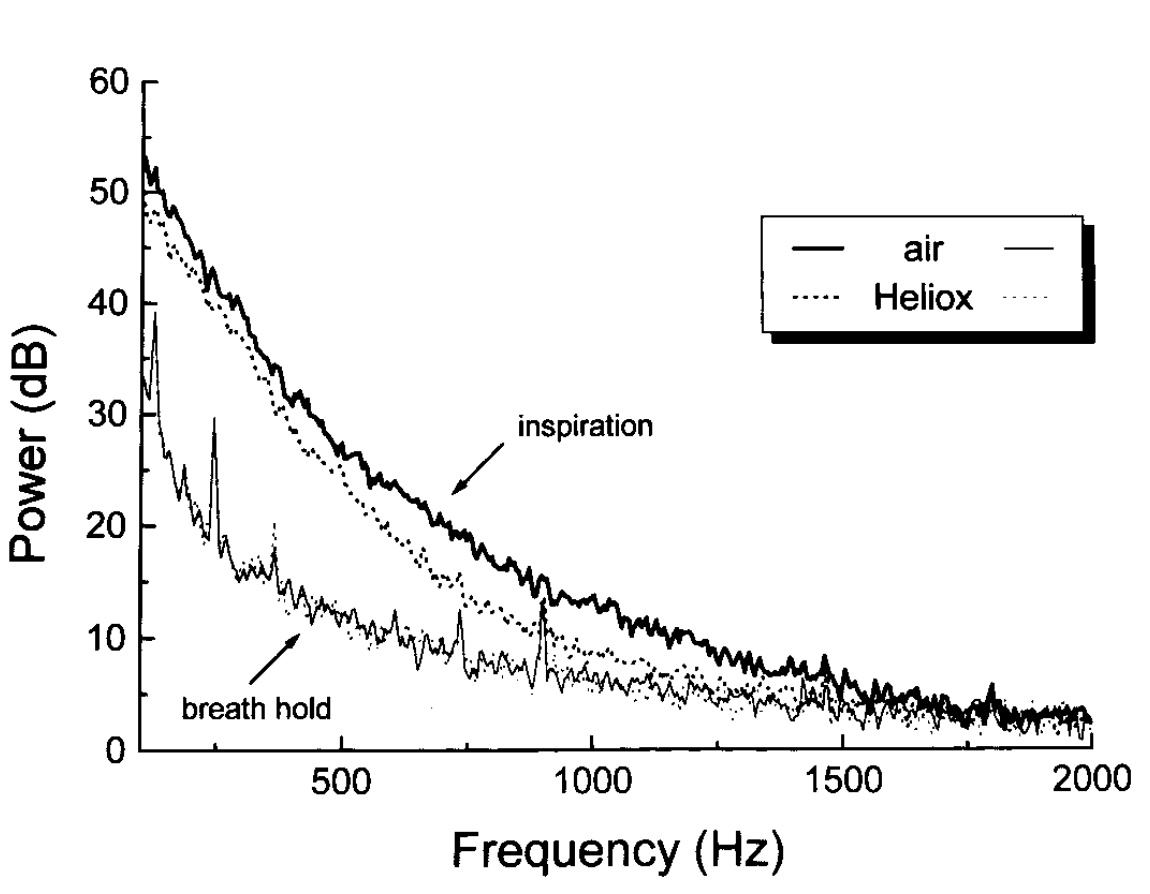
\includegraphics[width=\linewidth]{images/insp-spectrum.png}
\caption{Power spectra of normal lung sounds in a healthy adult male subject, recorded with a contact sensor over the superior right lower lobe}
\label{fig:left}
\end{subfigure}
\hfill
\begin{subfigure}[t]{0.4\textwidth}
\centering
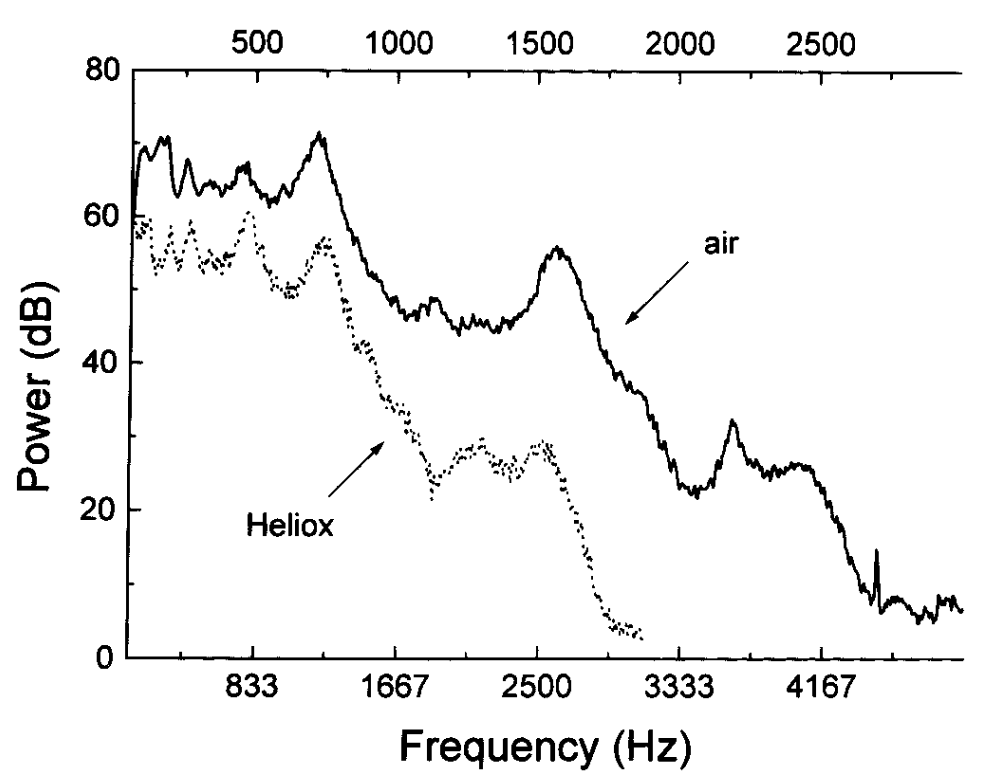
\includegraphics[width=\linewidth]{images/trache-Spectrum.png}
\caption{Power spectra of normal tracheal sounds in a healthy man, recorded with a contact sensor at the suprasternal notch }
\label{fig:right}
\end{subfigure}
\label{fig:double}
\caption{Graphs from H. Pasterkamp et al. \cite{pasterkamp_respiratory_1997}. Higher Frequency content can be observed in (b) due to the direct coupling to the airway lumen. \\ 
The additional graphs using Heliox show the parenchymal pathway is not affected by the change in gas density as sound is conveyed through the tissue.}
\end{figure}

Pathological conditions can produce additional sounds as listed in Table \ref{tab:resp_sounds}.
\begin{table}[H]
\centering
\footnotesize
\caption{Categories of Respiratory Sounds - adopted from \cite{pasterkamp_respiratory_1997}}
\label{tab:resp_sounds}

\begin{tabularx}{\textwidth}{lXXXX}
\toprule
\textbf{Respiratory Sound} & \textbf{Mechanisms} & \textbf{Origin} & \textbf{Acoustics} & \textbf{Relevance} \\
\midrule

\multicolumn{5}{l}{\textbf{Basic sounds}} \\
\addlinespace

Normal lung sound &
Turbulent flow vortices, unknown mechanisms &
Central airways (expiration), lobar to segmental airways (inspiration) &
Low-pass filtered noise (range $<100$ to $>1000$ Hz) &
Regional ventilation, airway caliber \\
\addlinespace

Normal tracheal sound &
Turbulent flow, flow impinging on airway walls &
Pharynx, larynx, trachea, large airways &
Noise with resonances (range $<100$ to $>3000$ Hz) &
Upper airway configuration \\
\midrule

\multicolumn{5}{l}{\textbf{Adventitious sounds}} \\
\addlinespace

Wheeze &
Airway wall flutter, vortex shedding &
Central and lower airways &
Sinusoid (range $\sim100$ to $>1000$ Hz; duration typically $>80$ ms) &
Airway obstruction, flow limitation \\
\addlinespace

Rhonchus &
Rupture of fluid films, airway wall vibrations &
Larger airways &
Series of rapidly dampened sinusoids (typically $<300$ Hz; duration $>100$ ms) &
Secretions, abnormal airway collapsibility \\
\addlinespace

Crackle &
Airway wall stress-relaxation &
Central and lower airways &
Rapidly damped wave deflection (duration typically $<20$ ms) &
Airway closure, secretions \\
\bottomrule
\end{tabularx}

\vspace{0.3cm}
\footnotesize{
* This table lists only the major categories of respiratory sounds and does not include other sound such as squawks, friction rubs, grunting, snoring, or cough. Current concepts on sound mechanisms and origin may be incomplete and unconfirmed
}
\end{table}

\section{Joints and Tendons}
Acoustic Emission (AE) of joints under load is widely considered to be a natural phenomenon \cite{whittingslow_acoustic_2020}. 
As Emissions are generated by the movement of the joint surfaces, this dynamic approach is the main advandtage over static mode examinations such as MRI or Ultrasound and can be correlated to joint angle and load.
By means of placing a sensor on the skin over bony prominence acoustic signals can be detected. 
Signals are generated by the interaction of the articular surfaces, ligaments and tendons and range up to \SI{500}{k\hertz} \cite{shark_discovering_2010}
\\In order to analyze the AE signal, it is common to to describe individual hits. A hit is defined as a transient, burst like event satisfying a set of definition parameters. 
The most commonly used parameters are the amplitude, duration and frequency content of the hit \cite{whittingslow_acoustic_2020}. A graphic overview is given in Fig. \ref{fig:AEhit}.
\begin{figure}
\centering
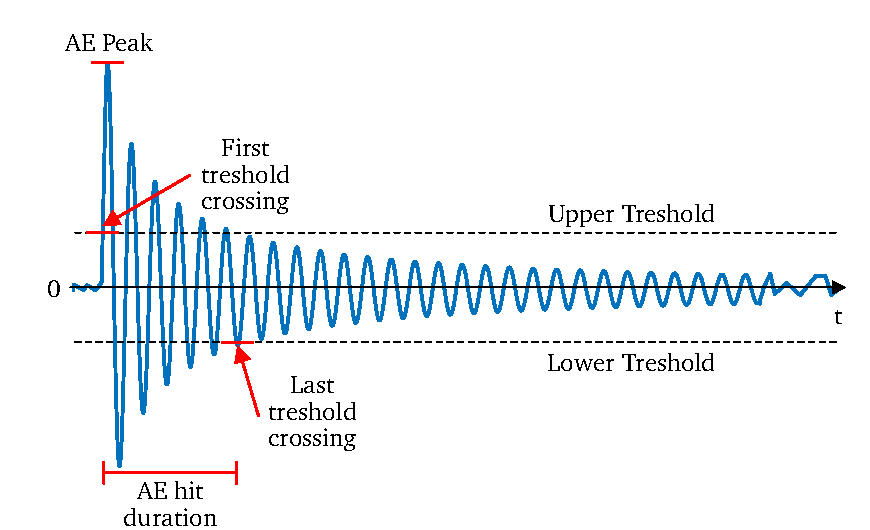
\includegraphics[width=0.8\textwidth]{images/AE HIT.pdf}
\caption{Graphic overview of the most commonly used parameters for describing and classifying an AE hit.}
\label{fig:AEhit}
\end{figure}

Another metric for assessing the health of cartilaginous joints is the analysis of the continuous activity summarized in the b-value \cite{jeong_b-value_2018}.

\begin{align}
\log_{10}(N_{AE}) &= a - bA_{dB}   \\
A_{dB} &= 20 \log_{10}\left(\frac{V_{\text{peak}}}{V_{\text{ref}}}\right)
\end{align}

The b-value is derived from the field of seismology, expressing the logarithmic relationship between magnitude and frequency of a shockwave generated by an earthquake. 
In the context of joints, the coefficient b describes the decrease in the number of hits $N_{AE}$ with an increasing amplitude $A_{dB}$ serving as the detection threshold.

\cite{jeong_b-value_2018} showed, that the b-value is significantly lower in patients with an injured knee (1.46 ± 0.35)(torn anterior cruciate ligaments, torn lateral menisci, and sprained medial collateral ligaments) compared to healthy controls (1.92 ± 0.2), meaning that more high amplitude hits are present. 
\cite{shark_discovering_2010} too observed a higher number of high amplitude hits in patients with osteoarthritis compared to healthy controls. 




\section{Muscle Sounds}

\chapter{Sensor Types}
A typical AE monitoring system (Fig. 1, top) takes its input from an AE sensor that converts dynamic surface motion into electric signals [6]. 
Due to the low amplitude of AE signals and the high impedance of piezoelectric sensors, the amplification is usually carried out in two steps, firstly by the pre-amplifier and subsequently by the main amplifier. Band pass filters are also employed to eliminate unwanted noise, such as sensor and electrical circuit noise, electromagnetic interference, background and technological acoustics noise. 
\section{Low Frequency Sensors}
\subsection{Seismographic Sensors}
\section{High Frequency Sensors}
\subsection{Piezoelectric Sensors}
\section{Ferroelectret Sensors }
\chapter{Discussion}



\chapter{Conclusion}


\printbibliography

\end{document}
